\documentclass[master.tex]{subfiles}
\begin{document}

\chapter{Example Formal System - Typed Lambda Calculus}
\label{chap:example_lambda_calculus}

Chapters \ref{chap:example_simple_arithmetic} and
\ref{chap:example_propositional_logic} show most of features and usability of
\emph{Phometa} already so this chapter aims to show that Phometa is powerful
enough as it can even encode more complex formal system like \emph{typed lambda
  calculus}. Hence, it is clear that Phometa is suitable to encode most of
formal system that user can think of.

Please note that, this formal system encoded in the standard library of Phometa
is partly complete due to project time frame constrain. Currently, only
$\beta$-reduction and simply type are implemented here.

Credit: Some of material here modified from lecture note of ``382 --- Type
Systems for Programming Languages'' (third year course), Department of
Computing, Imperial College London. Thank you Dr Steffen van Bakel for this.

TODO: write an explanation for each screenshot.

\section{Terms and Variables}

\begin{figure}[H]
    \centering
\begin{minipage}{0.7\textwidth}
    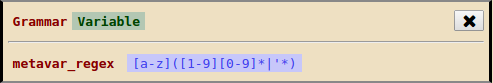
\includegraphics[width=\textwidth]{lamb-gmr-var}
    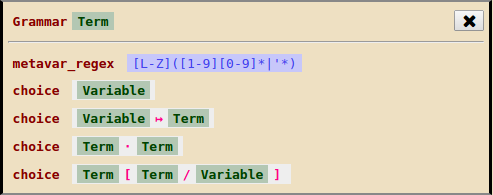
\includegraphics[width=\textwidth]{lamb-gmr-term}
\end{minipage}
\caption{Definition of \pgmr{Variable} and \pgmr{Term}}
\end{figure}
\section{Side Conditions}
Sometime we want to build a simple formal system but its dependency relies on
more complex formal system, for example, $\beta$ reduction needs to check
weather a variable is a free variable of a curtain term or not, and checking
free variable require knowledge of set. Normally we should build a formal system
regarding to set first then we can build $\beta$ reduction, however this is
overkill as formal system is much larger than $\beta$ reduction. To solve this
problem, we can build a grammar that construct a statement that represent
whether a variable is a free variable of a certain term or not as the following

\begin{figure}[H]
    \centering
\begin{minipage}{0.7\textwidth}
    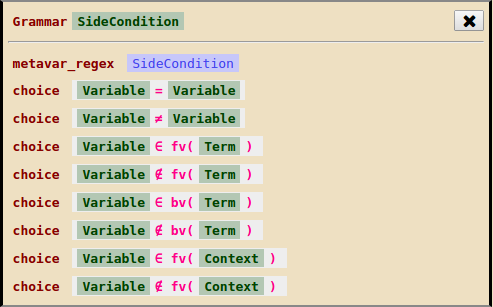
\includegraphics[width=\textwidth]{lamb-gmr-sidecond}
\end{minipage}
\caption{Definition of \pgmr{SideCondition}}
\end{figure}

Then write a single rule that allow to prove any side condition.

\begin{figure}[H]
    \centering
\begin{minipage}{0.7\textwidth}
    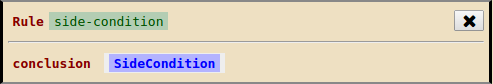
\includegraphics[width=\textwidth]{lamb-rule-sidecond}
\end{minipage}
\caption{Definition of \prule{side-condition}}
\end{figure}

Every time when \pgmr{SideCondition} appear in a derivation tree, user needs
extra care and determine whether that side condition holds or not. If it holds
then apply \prule{side-condition} and it is done. Please note that there is no
mechanism to prevent user to apply \prule{side-condition} on a false
\pgmr{SideCondition} and it will result in inconsistency, in another word, by
using side condition technique, we \emph{trust} user to do the right thing.

\section{$\beta$ Reduction}

\begin{figure}[H]
    \centering
\begin{minipage}{0.7\textwidth}
    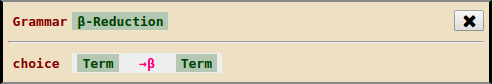
\includegraphics[width=\textwidth]{lamb-gmr-beta}
\end{minipage}
\caption{Definition of \pgmr{$\beta$-Reduction}}
\end{figure}

\begin{figure}[H]
    \centering

\begin{minipage}{0.48\textwidth}
\begin{flushleft}
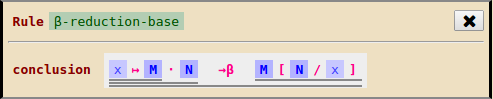
\includegraphics[width=\textwidth]{lamb-rule-beta-1}
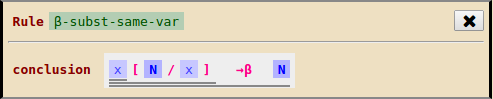
\includegraphics[width=\textwidth]{lamb-rule-beta-2}
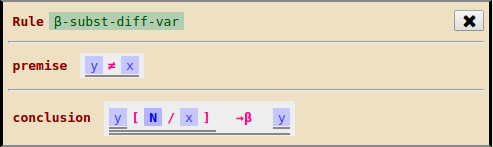
\includegraphics[width=\textwidth]{lamb-rule-beta-3}
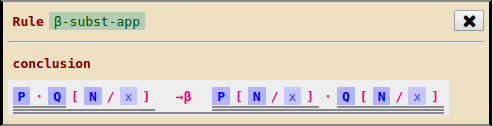
\includegraphics[width=\textwidth]{lamb-rule-beta-4}
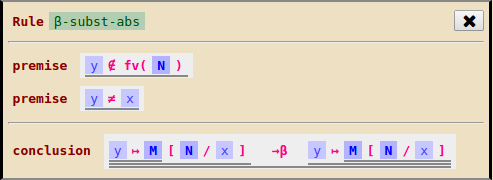
\includegraphics[width=\textwidth]{lamb-rule-beta-5}
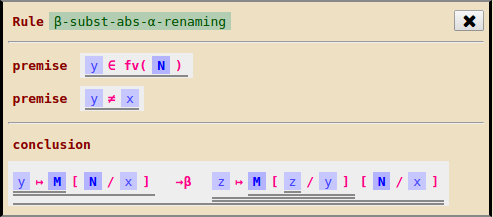
\includegraphics[width=\textwidth]{lamb-rule-beta-6}
\end{flushleft}
\end{minipage}
~
\begin{minipage}{0.48\textwidth}
\begin{flushright}
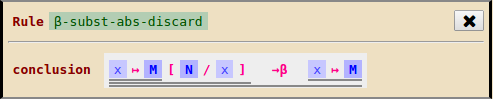
\includegraphics[width=\textwidth]{lamb-rule-beta-7}
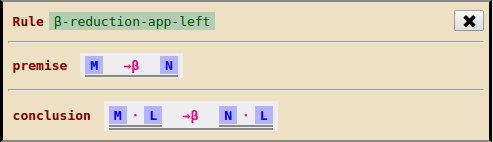
\includegraphics[width=\textwidth]{lamb-rule-beta-8}
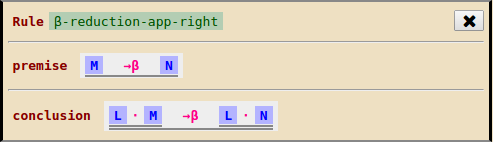
\includegraphics[width=\textwidth]{lamb-rule-beta-9}
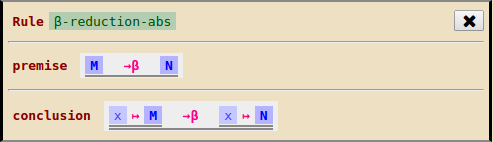
\includegraphics[width=\textwidth]{lamb-rule-beta-10}
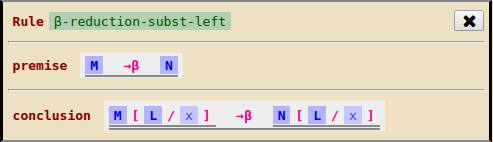
\includegraphics[width=\textwidth]{lamb-rule-beta-11}
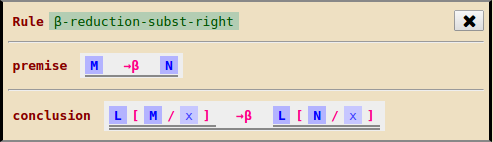
\includegraphics[width=\textwidth]{lamb-rule-beta-12}
\end{flushright}
\end{minipage}

    \caption{Rules for \pgmr{$\beta$-Reduction}}
\end{figure}


\begin{figure}[H]
    \centering
\begin{minipage}{0.48\textwidth}
\begin{flushleft}
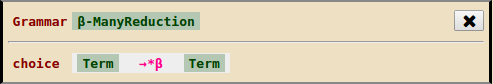
\includegraphics[width=\textwidth]{lamb-gmr-betamany}
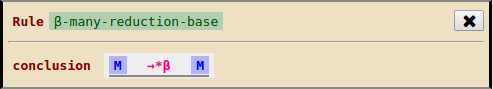
\includegraphics[width=\textwidth]{lamb-rule-betamany-1}
\end{flushleft}
\end{minipage}
~
\begin{minipage}{0.48\textwidth}
\begin{flushright}
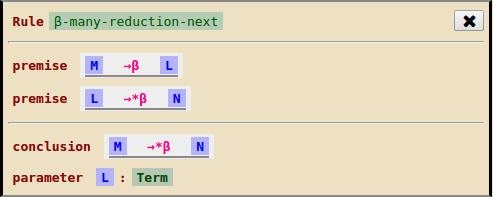
\includegraphics[width=\textwidth]{lamb-rule-betamany-2}
\end{flushright}
\end{minipage}

\caption{Definition of \pgmr{$\beta$-ReductionMany and its rules}}
\end{figure}

\section{Simply Types}


\begin{figure}[H]
    \centering
\begin{minipage}{0.7\textwidth}
    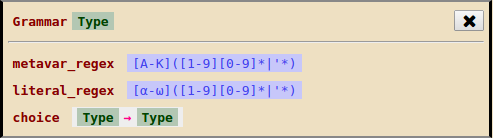
\includegraphics[width=\textwidth]{lamb-gmr-type}
    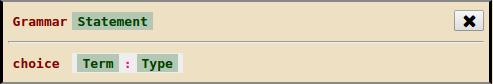
\includegraphics[width=\textwidth]{lamb-gmr-statement}
    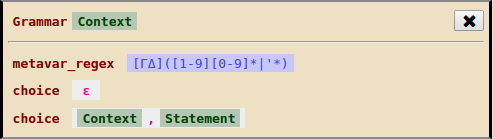
\includegraphics[width=\textwidth]{lamb-gmr-context}
    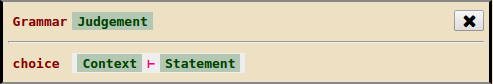
\includegraphics[width=\textwidth]{lamb-gmr-judgement}
\end{minipage}
\caption{Definition of grammars related to \pgmr{Type}}
\end{figure}


\begin{figure}[H]
    \centering
\begin{minipage}{0.7\textwidth}
    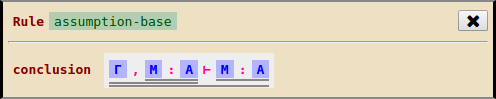
\includegraphics[width=\textwidth]{lamb-rule-type-1}
    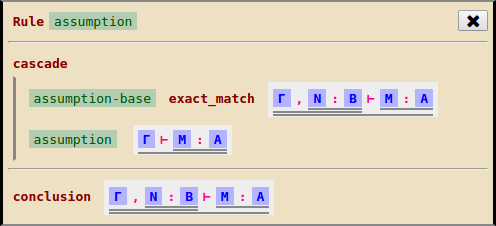
\includegraphics[width=\textwidth]{lamb-rule-type-2}
    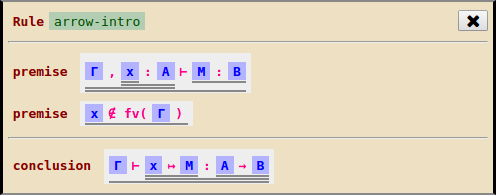
\includegraphics[width=\textwidth]{lamb-rule-type-3}
    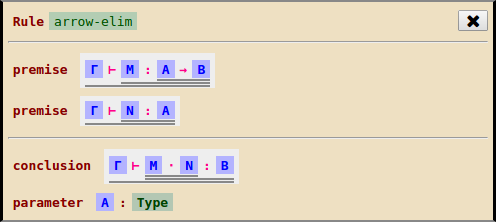
\includegraphics[width=\textwidth]{lamb-rule-type-4}
\end{minipage}
\caption{Definition of rules using for type resolution.}
\end{figure}

\end{document}